\section{Implementacja}
Rozdział ten opisuje działanie pojedynczego węzła bez zagłębiania się w szczegóły jego architektury. Węzeł jest samodzielną aplikacją. Może więc działać bez obecności innych węzłów. Sam stanowi wtedy jedyny punkt w systemie i przesyła zapytania sam do siebie. Taka konfiguracja, choć mało praktyczna, jest możliwa.



\subsection{Cykl życia instancji}
Administrator ma możliwość swobodnego włączania i wyłączania nowych węzłów. Po uruchomieniu węzła (aplikacji), uruchamiany jest supervisor. Uruchamia on kolejno wszystkie gen\_servery:, w kolejnośći:
\begin{enumerate}
	\item storage\_uuid\_srv
	\item storage\_core\_srv
	\item storage\_auth\_srv
	\item storage\_dist\_srv
	\item storage\_http\_srv
\end{enumerate}

Każdy uruchomiony jest w trybie one-for-one – w przypadku awarii jednego z nich, tylko on zostanie uruchomiony ponownie. Maksymalna liczba prób ponownego uruchomienia dla każdego gen\_servera wynosi 5. Po przekroczeniu tej liczby, uznaje się, że awaria jest krytyczna.

Kolejność uruchamiania może być dowolna – procedury inicjalizacyjne poszczególnych serwerów nie zależą od dostępności innych. Należy jednak mieć na uwadze, że uruchomienie serwera storage\_dist\_srv spowoduje, że system będzie mógł przyjmować komunikaty od użytkowników, więc storage\_core\_srv powinien już działać.

Wszystkie zmiany w metadanych plików są persystowane w bazie danych. Po wyłączeniu / awarii węzła i ponownym jego włączeniu, zapisane dane zostają odtworzone. Jeżeli jakieś zapytanie było w kolejce wątku wykonawczego który został zatrzymany, zapytanie zostaje zgubione i użytkownik musi wykonać je ponownie.

Jeżeli węzeł nie przeprowadza aktualnie żadnych operacji, może zostać bezpiecznie wyłączony.



\subsection{Wewnętrzne protokoły}
Istnieją procedury wymagające współpracy wielu węzłów, bardziej skomplikowane niż przykładowo tworzenie pliku w systemie. Jedna z nich to procedura dołączania nowego węzła do systemu, w wyniku której każdy węzeł w systemie dysponuje aktualnym jego obrazem i jest poinformowany o dołączeniu nowego węzła. Druga z procedur ma miejsce, kiedy dochodzi do autentykacji zapytania. Dane użytkowników są przechowywane w różnych węzłach i mogą ulegać zmianom w czasie, dlatego należy dokonać takiego wyszukiwania w optymalny sposób ograniczając liczbę przesyłanych wiadomości.

\subsubsection{Dołączanie węzłów (synchronizacja stanu)}
Każdy węzeł na starcie pobiera z pliku konfiguracyjnego lokalizację (adres) węzła początkowego (initial node). Jest to węzeł działający w klastrze, do którego dołączany jest nowy węzeł. Może to być również adres własny jeżeli węzeł ma działać samodzielnie / być pierwszym węzłem w klastrze.

Nowy węzeł w trakcie uruchamiania rozpoczyna procedurę \textit{remote scan} (storage\_dist\_srv:remote\_scan/1). Wykonywana jest w trakcie inicjalizacji modułu storage\_dist\_srv. \autoref{fig:sync-state-seq} pokazuje przebieg sekwencji wywołań i komunikatów tej procedury.

\begin{figure}[!htbp]
	\centering
	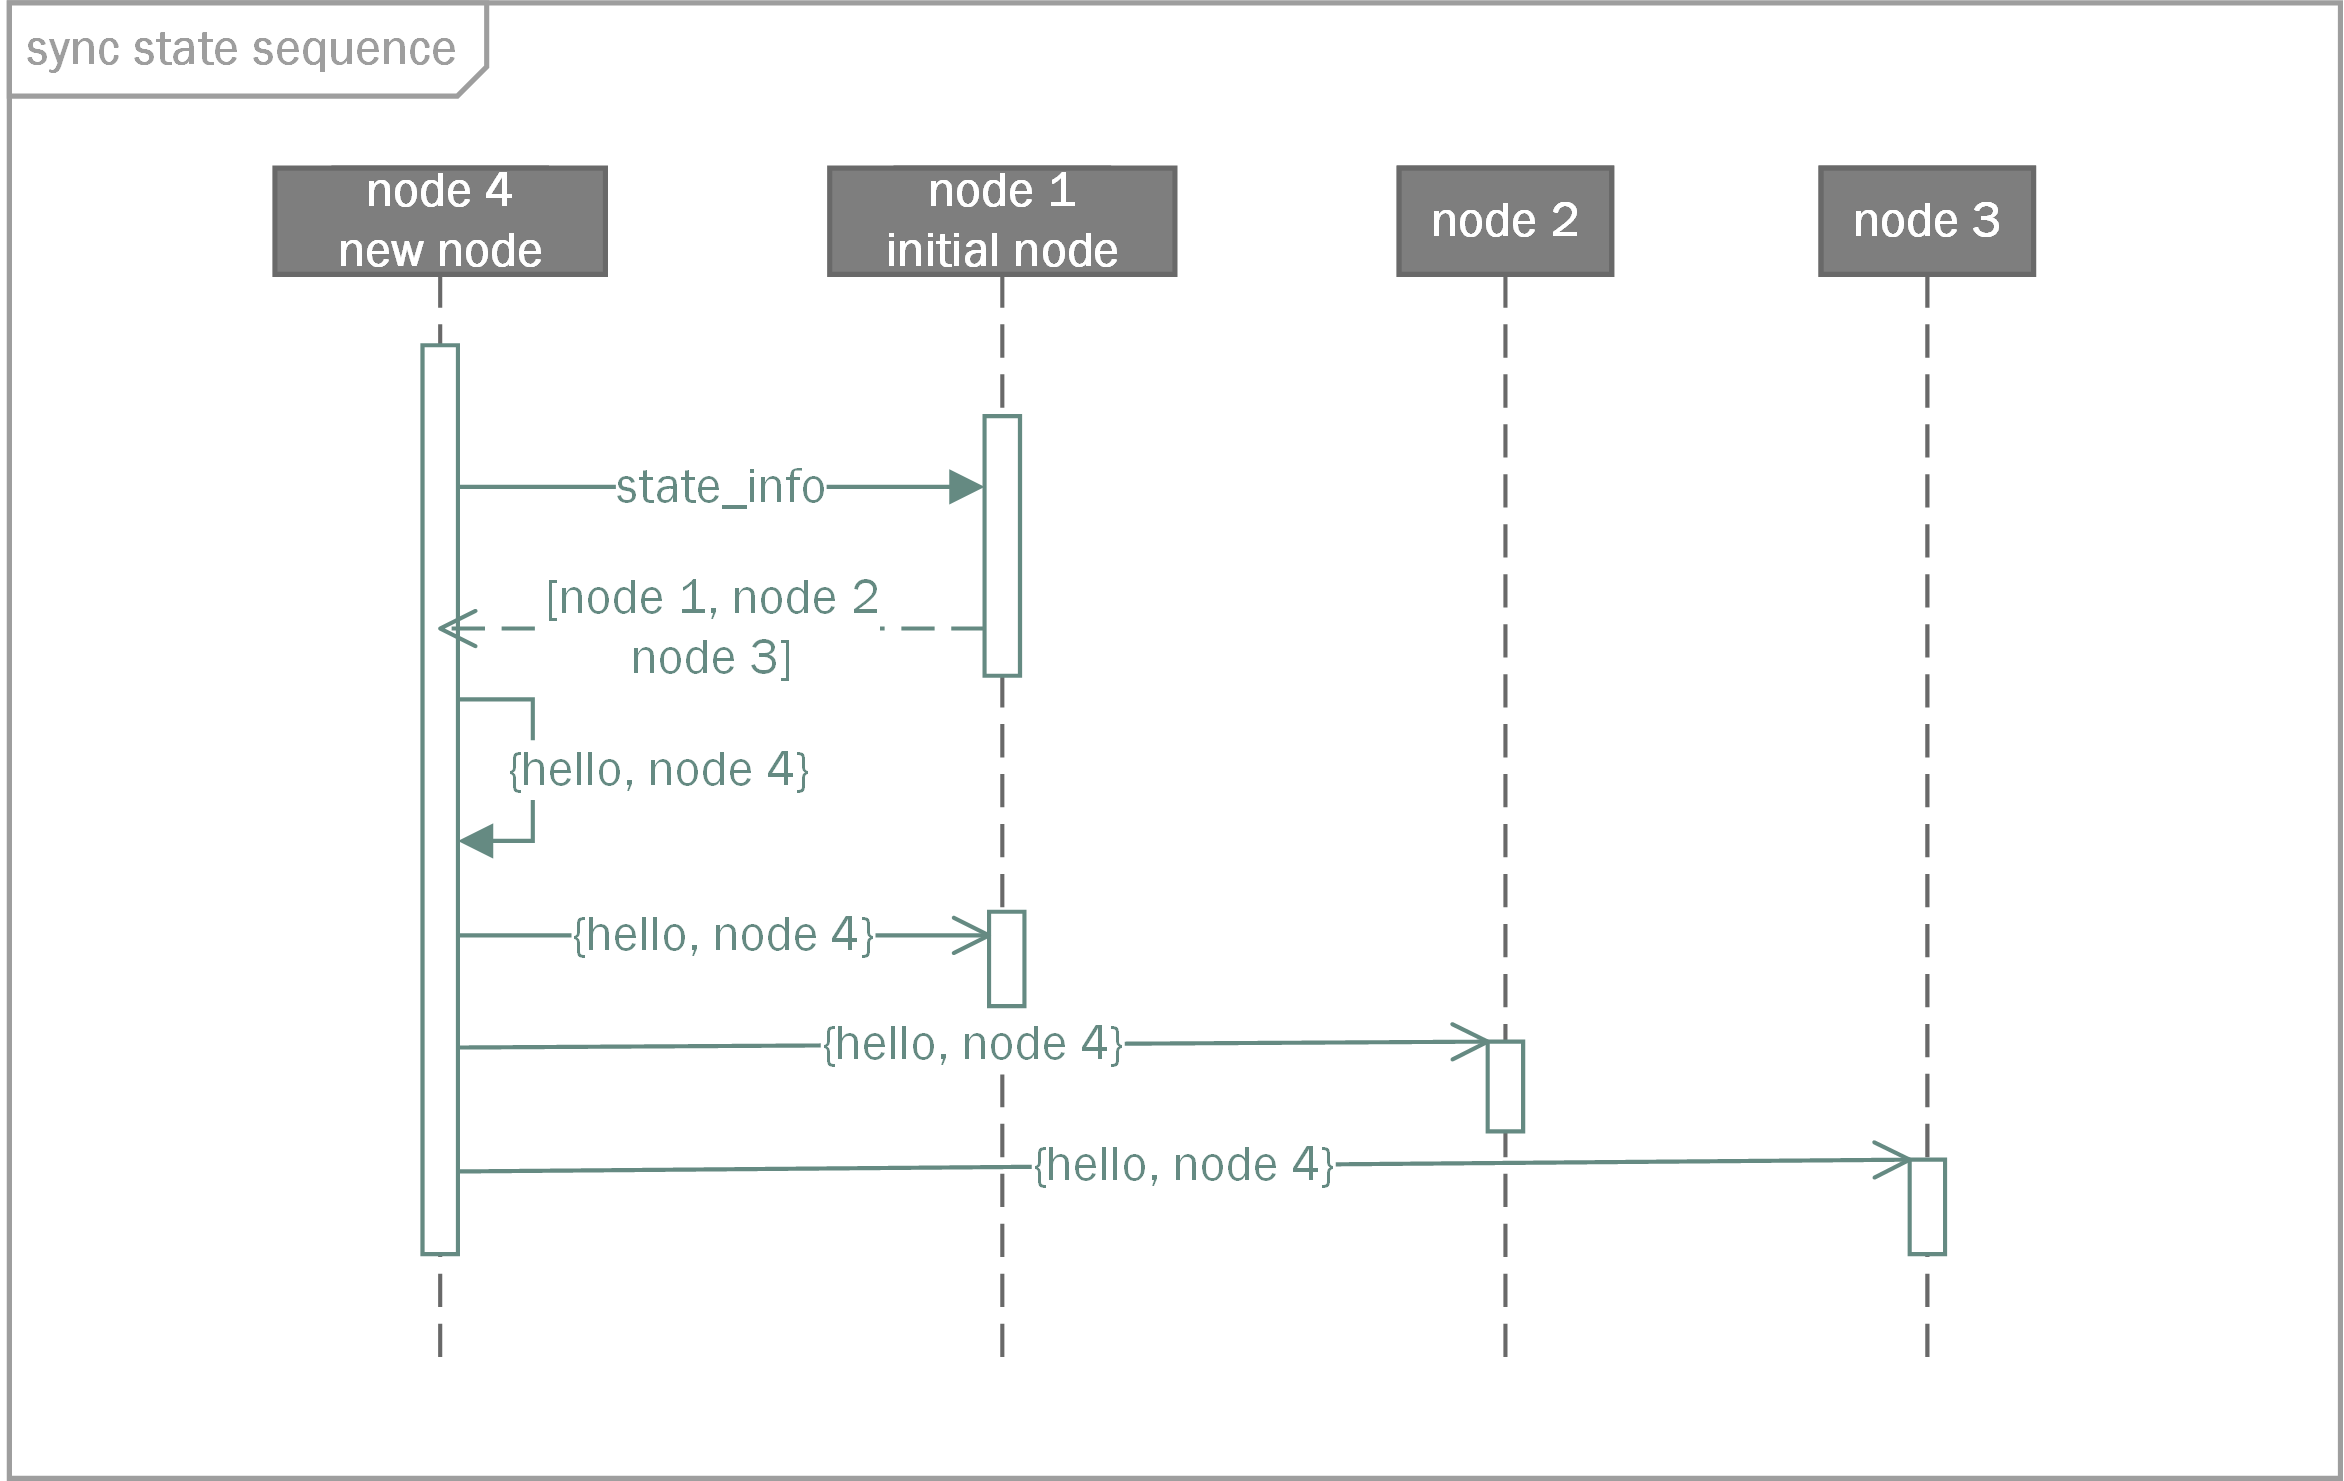
\includegraphics[width=0.9\textwidth]{sync-state-seq}
	\caption[Synchronizacja listy węzłów.]{Synchronizacja listy węzłów. Uproszczony wariant z jednym initial node.}
	\label{fig:sync-state-seq}
\end{figure}

Przyjmuje ona zbiór adresów węzłów (domyślnie znajduje się tam tylko initial node). Ze zbioru usuwany jest aktualny węzeł (zbiór może przez to stać się pusty). Następnie do każdego serwera storage\_dist\_srv działającego na każdym z węzłów ze zbioru wysyłany jest komunikat (atom) state\_info. Odpowiedzią na ten komunikat jest zwrócenie pytającemu informacji o znanych sobie węzłach w postaci listy. Domyślny węzeł łączy te listy w jedną, z której następnie usuwa duplikaty.

Ten nowy zbiór staje się stanem nowego węzła i będzie udostępniany w wywołaniach state\_info kierowanych do niego. Ostatnim krokiem jest rozesłanie do wszystkich poznanych węzłów komunikatu \{hello, node()\} z własnym adresem. Każdy z nich uaktualni wtedy listę znanych sobie węzłów o nowy węzeł.





\subsubsection{Synchronizacja użytkowników}
Użytkownicy przechowywani są w węźle, na którym zostało utworzone ich konto (dodane do bazy danych). Ponieważ użytkownik może wykonywać zapytania wysyłając je do dowolnego węzła, należy zapewnić możliwość uzyskania dostępu do danych użytkownika bez informacji o tym, na którym węźle znajdują się informacje o jego koncie.

Informacją niezbędną do autentykacji zapytania jest klucz prywatny użytkownika. Moduł storage\_auth\_srv działający na każdym węźle zarządza listą krotek \{username, secret, expires\}. Taka struktura wystarcza żeby dokonać autentykacji użytkownika.

Kiedy storage\_auth\_srv autentykuje zapytanie, szuka użytkownika w opisanej wyżej liście. Jeżeli go znajdzie, wykorzystuje skojarzony klucz prywatny do wyliczenia sumy kontrolnej. Jeżeli nie ma takiego użykownika, wysyła zapytanie rozgłoszeniowe do wszystkich innych modułów storage\_auth\_srv. Odpowiada na nie węzeł, który znajdzie w swojej bazie danych szukanego użytkownika. Po pewnym czasie lista zapełni się użytkownikami i nie będzie trzeba sięgać do innych węzłów w celu autentykacji zapytania.

Dane użytkownika mogą się zmienić (może na przykład zmienić hasło). By w systemie nie zalegały nieaktualne dane, każdy rekord ma dodatkowo pole expires, które ustawiane jest domyślnie na 10 minut. Przedawnione wpisy są traktowane na równi z brakiem wpisów w liście użytkowników.

Jeżeli walidacja przy pomocy przechowywanego w liście klucza nie powiedzie się, istnieje przypuszczenie, że użytkownik zmienił swoje hasło i podpisał wiadomość nowym kluczem. W takim wypadku komunikat z poszukiwaniem użytkownika jest jeszcze raz rozgłaszany w systemie.

\begin{figure}[!htbp]
	\centering
	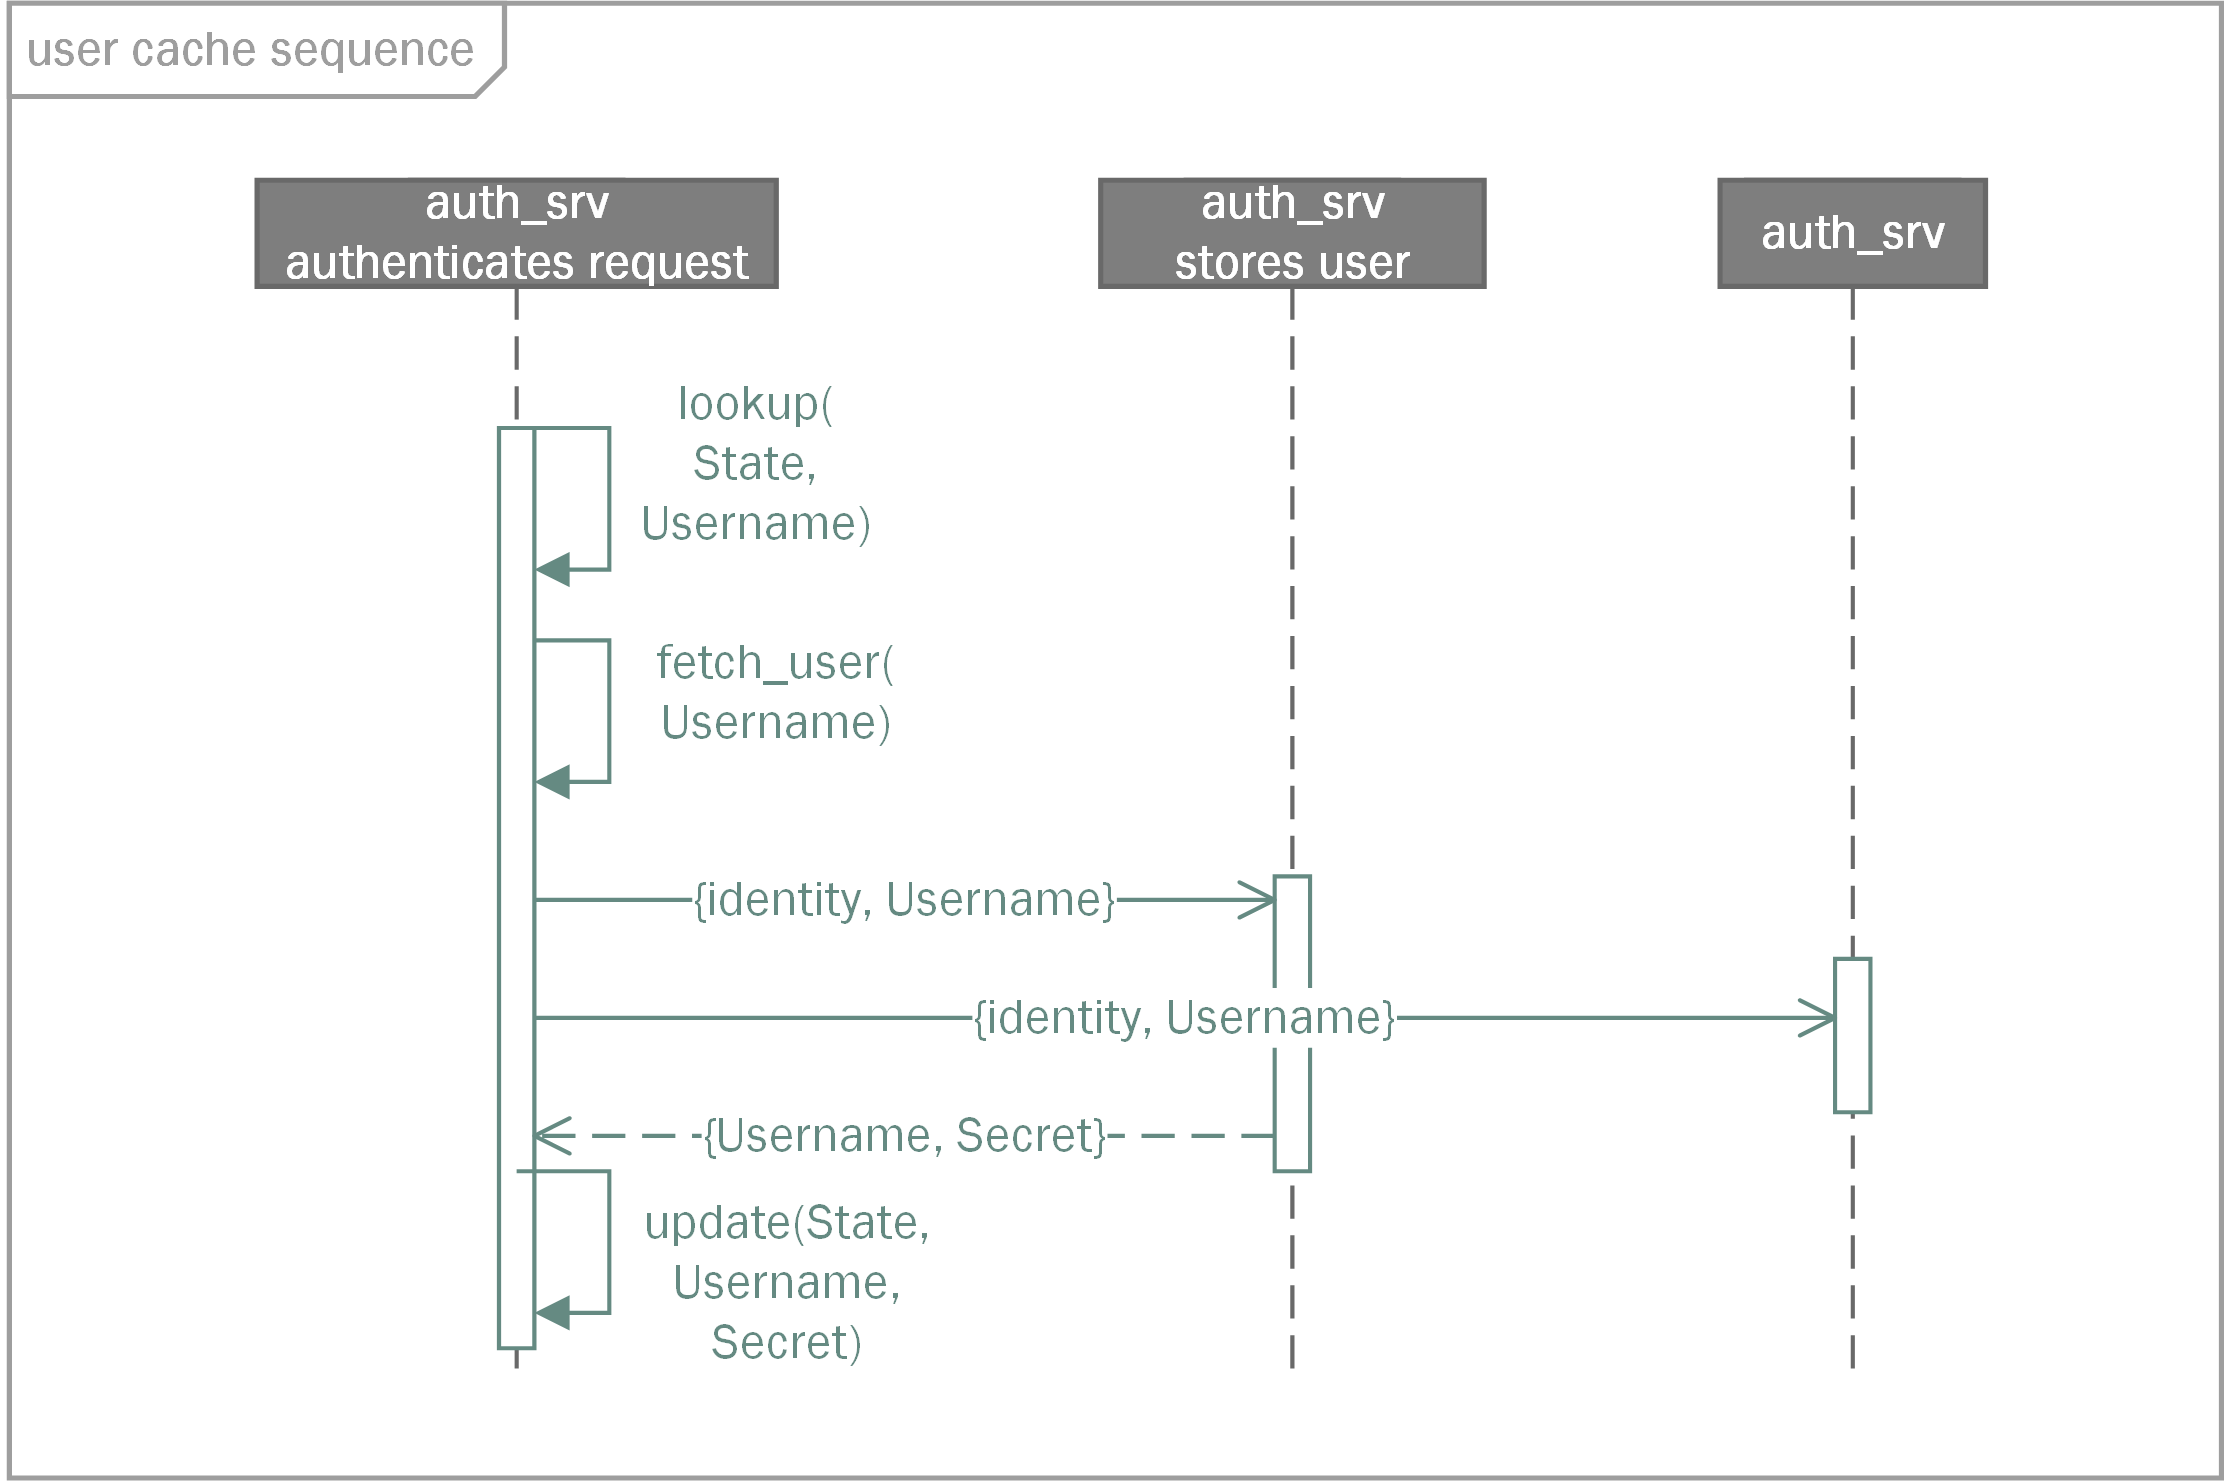
\includegraphics[width=0.9\textwidth]{user-seq}
	\caption[Wyszukiwanie użytkownika w systemie.]{Wyszukiwanie użytkownika w systemie. Użytkownik nie zostaje znaleziony w lokalnym cache. Rozgłaszany jest komunikat {identity, Username}. Odpowiedni węzeł zwraca informacje na temat użytkownka lista cache ulega aktualizacji.}
	\label{fig:user-seq}
\end{figure}